\cleartooddpage[\thispagestyle{empty}]
\chapter{The VERITAS Observatory}\label{chapter:veritas}

\begin{figure}[ht]
  \centering
  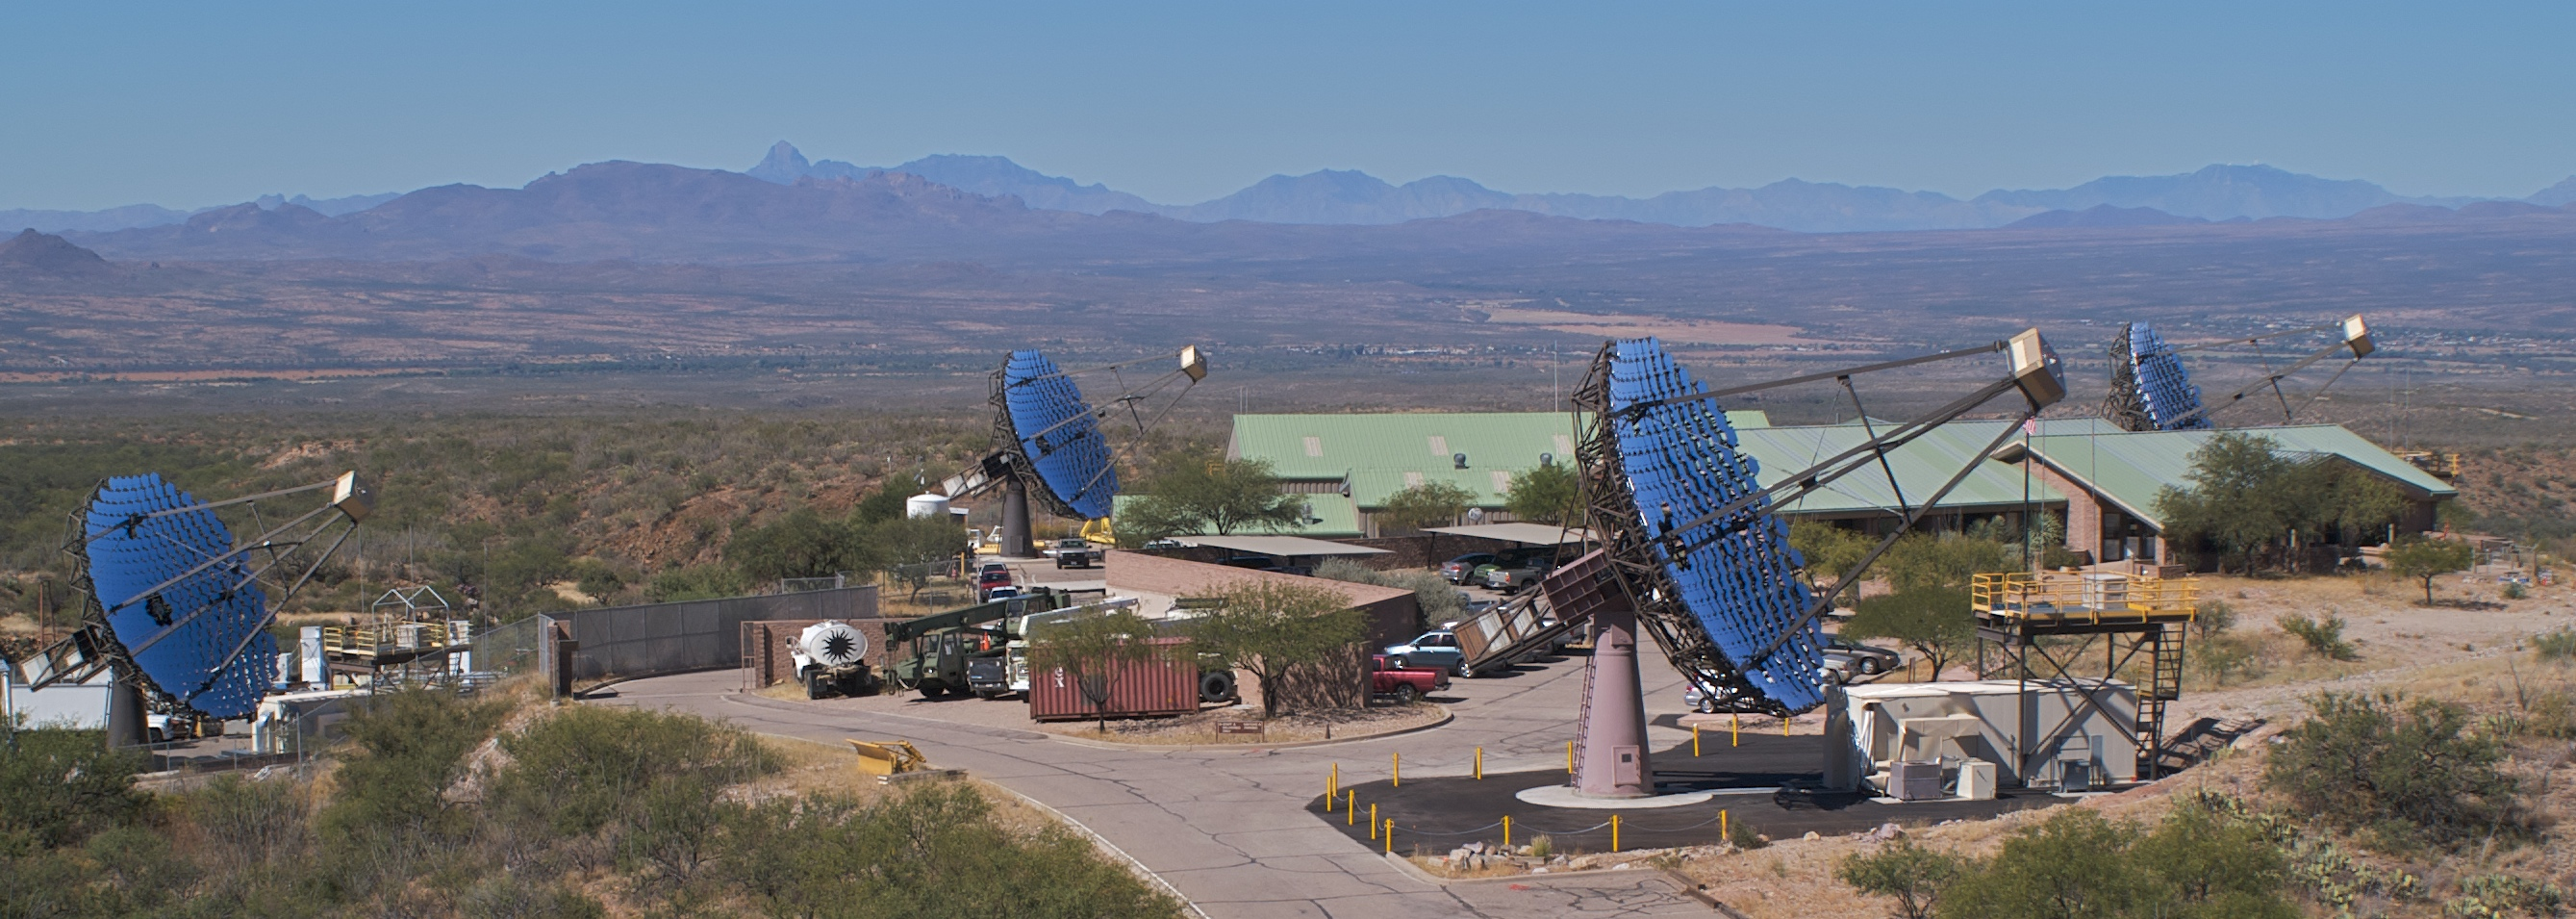
\includegraphics[width=0.95\textwidth]{images/veritas_array_v6}
  \caption[VERITAS Array]{
    The VERITAS observatory.}
  \label{fig:veritasarray}
\end{figure}

VERITAS, or Very Energetic Radiation Imaging Telescope Array System pictured in Figure~\ref{fig:veritasarray}, is a gamma ray observatory operating in Arizona, USA, and is capable of detecting \nicetilde{}\TeV{} gamma rays.
The observatory consists of an array of four Imaging Atmospheric Cherenkov Telescopes (IACTs), each spaced \nicetilde{}\SI{90}{m} apart.
Each telescope possesses an array of 345 mirrors, and a 499 Photomultiplier Tube (PMT) camera on a set of struts.
When a gamma ray produces an air shower in the atmosphere, the shower emits blue-UV Cherenkov photons over a timespan of nanoseconds.
By focusing these photons onto the PMT camera with the mirrors, images of the shower can be taken, in which each pixel of the image consists of analog voltage pulses from each PMT.


The different hardware components are examined in this chapter, in order of signal propagation.
Section~\ref{sec:telpoint} details the Telescope Pointing, including its monitoring and calibration.
The Mirrors are discussed in Section~\ref{sec:mirrors}, including their properties and alignment.
In Section~\ref{sec:pmts}, the PMTs are explored, including their performance and calibration.
The trigger system is examined in Section~\ref{sec:trig}, relating how candidate signal voltages are saved while discarding those sourced from noise.
Section~\ref{sec:epochs} relates the different observatory epochs, as over time changes and modifications have altered the observatory's performance.


\section{Telescope Pointing}\label{sec:telpoint}

\begin{figure}[ht]
  \centering
  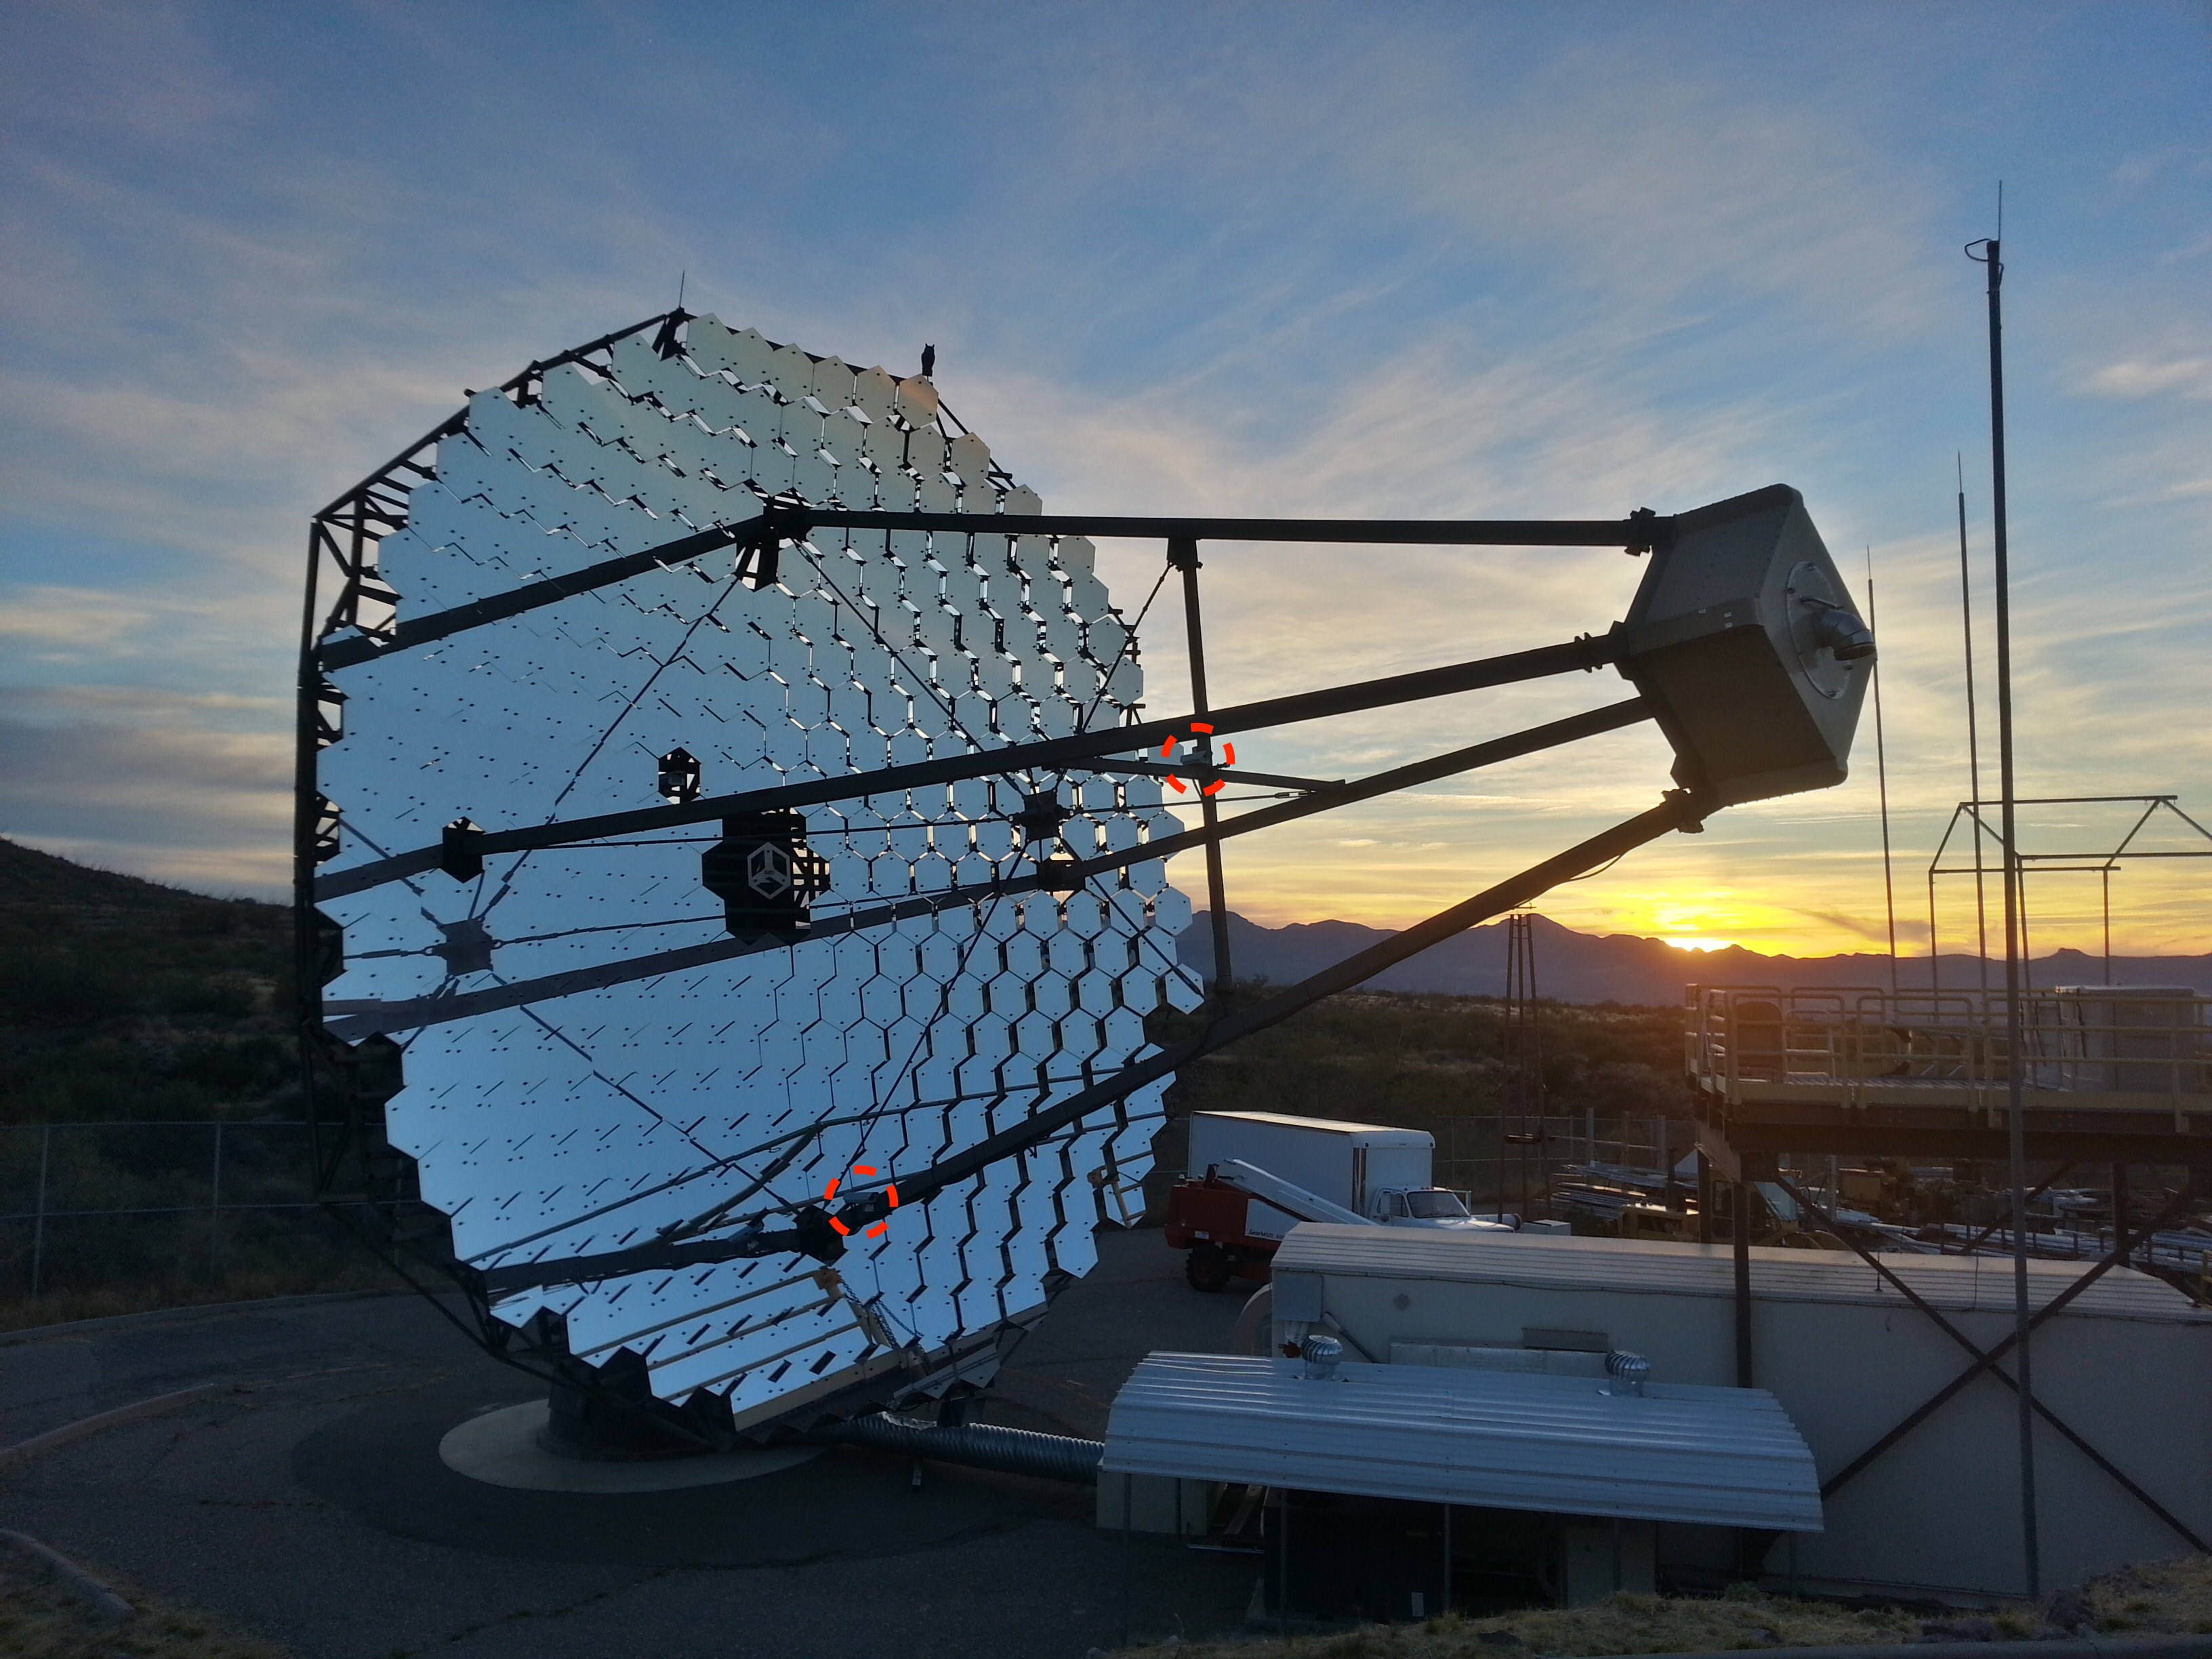
\includegraphics[width=0.95\textwidth]{images/single_telescope}
  \caption[Single Veritas Telescope]{
    View of the 345 mirrors, the support structure, and the PMT Camera housing at the end of the four supporting arms.}
  \label{fig:davcottel}
\end{figure}

Like most telescopes, each VERITAS telescope has a fixed base and a pointable dish for collecting light.
This dish can rotate in azimuth and in elevation, with enough range in both axes to point at any direction above the horizon that is not blocked by local mountains.
At their fastest, the telescopes slew at a rate of \nicetilde{}\ang{1} per second.
To track where the telescopes are pointing, the motors that drive the azimuth and elevation movement have encoders that digitize the pointing direction of the dishes.
These encoders are attached to the axes of the motors, and thus they are capable of tracking the azimuth and elevation over its entire range of motion.
However, as the dishes are large metal structures, they bend and flex at different elevations and azimuths.
This flexing also posesses hysteresis, where the bending changes whether approching a pointing target from a higher or lower elevation.
To account for this flexing, the encoder values are then given to a structural model called T-Point, which corrects for the dish structure bending at different azimuths and elevations.
After applying this model, the telescope pointing can be tracked with an accuracy of \nicetilde{}\ang{0.02}~\cite{holder2008status}.
% jeff grube memo http://veritash.sao.arizona.edu:8081/AnalysisAndCalibration/111221_033051/VPM_memo_Dec2011.pdf ?
% or maybe just use https://arxiv.org/pdf/0810.0474.pdf ?

As an improvement to the encoder measurements, a VERITAS Pointing Monitor (VPM) system is also in place.
The VPM consists of two CCD cameras and 4 LED lights affixed to each telescope.
The CCD cameras are oriented such that they can view the PMT camera and the background stars.
The LED lights are attached to the PMT camera, next to the Winston cones, detailed in Section~\ref{sec:pmts}.
The first CCD camera is attached below the bottom mirrors, and images the stars in the field of view.
The second CCD camera is attached to the support struts, roughly halfway between the mirrors and the camera, and images the focal plane of the telescope.
Both cameras are marked by red dashed-line circles in Figure~\ref{fig:davcottel}.
During regular observations, these cameras take images of background stars and the focal plane LEDs every two seconds.
By extrapolating the LED positions from the star positions {\color{red}(is this how it works?? its unclear from the VPM memo...)}, an improved pointing accuracy of \nicetilde{}\ang{0.007} can be achieved~\cite{VPMmemo}.
%  0.007 comes from Grube 2011 VPM Memo:
%    20 arcseconds systematic error on VPN calibration (Section 3, last paragraph, and section 5 last paragraph)
%    +5 arcseconds due to scatter of star database positions (Section 5 last paragraph)
%    = 25 arcseconds total VPM systematic error
%
%    25 arcseconds -> 25/3600 -> 0.006944 deg -> rounded to 0.007 deg
This improvement persists down to an elevation of \ang{30}, where the data analysis in this thesis takes place.

\section{Mirrors}\label{sec:mirrors}

When the Cherenkov light from a gamma-ray shower first interacts with the telescope array, it is reflected by some of the 345 mirrors.
These mirrors face towards the incoming Cherenkov light, with the PMT camera facing the mirrors, as shown in Figure~\ref{fig:davcottel}.
When its spherical mirrors, spherical dish, and focal length ratio of \nicetilde{}2 are considered, this configuration is referred to as a Davies-Cotton telescope~\cite{daviescotton}.
Each mirror has an area of \SI{0.322}{m$^2$}, and a spherical curvature radius of \SI{24}{m}.
The mirrors are each mounted along the support structure so that the total diameter of the telescope's mirror area is \SI{12}{m}, with a total area of \SI{111}{m$^2$} and a focal length of \SI{12}{m}~\cite{Veritas_Detector}.
Figure~\ref{fig:mirreflect} shows the mirrors' reflectivity as a function of wavelength.
The VERITAS specifications state that the mirror reflectivity must be $\geq 85\%$, between \SIrange{280}{450}{nm}.

\begin{figure}[ht]
  \centering
  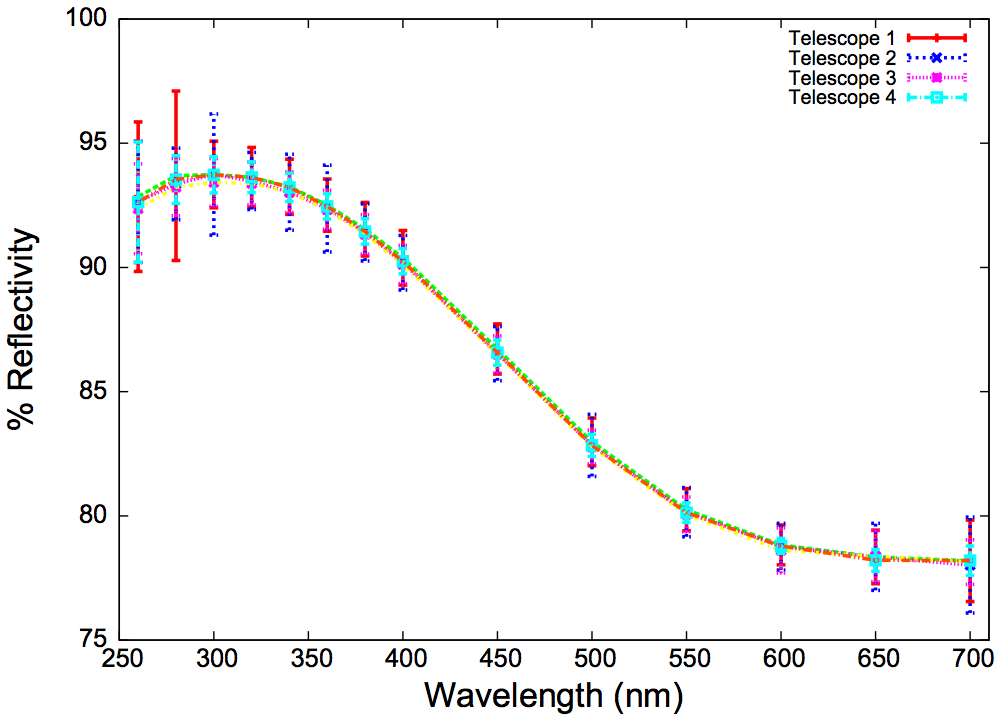
\includegraphics[width=0.75\textwidth]{images/mirror_reflect}
  \caption[Mirror Reflectivity]{
    Mirror reflectivity as a function of wavelength for each telescope, from Ref.~\cite{mirrorfacets}. 
    The lines are almost identical as each is an average over each telescope's 345 mirrors.
  }
  \label{fig:mirreflect}
\end{figure}

As the mirrors are exposed to the elements, they slowly accumulate dust and scratches.
To combat this, they are cleaned and recoated every two years.
Each mirror is attached to the support structure via three adjustable mounting points, allowing for adjustment of the mirror orientation to point directly at the camera, as detailed in~\cite{mirroralign}.
This alignment is measured and adjusted at regular intervals, using background stars as a calibration source.

\subsection{Star Point Spread Function}

Due to dust, minor imperfections in the surface of the mirrors, and small mirror misalignments, the photons that bounce off the mirrors are not reflected perfectly.
Instead, a single point-like light source appears blurred out on the focal plane.
This blurring is quantified by a fitted gaussian function, usually called the Optical Point Spread Function\footnote{Please note that this is different from the PSF described in Chapter \ref{ch:grrecon}, which quantifies the spread in the reconstructed gamma-ray positions.  The OPSF instead describes the spread of UV-Optical photons.} (OPSF).
By pointing a telescope at different stars and placing a CCD at the focal plane, the OPSF is measured monthly.
Figure~\ref{fig:mirrorpolaris} shows a calibration image from the first VERITAS telescope.
The OPSF is roughly gaussian-shaped but with longer tails and a $ \ang{0.06} $ full width half maximum~\cite{Veritas_Detector}.

\begin{figure}[ht]
  \centering
  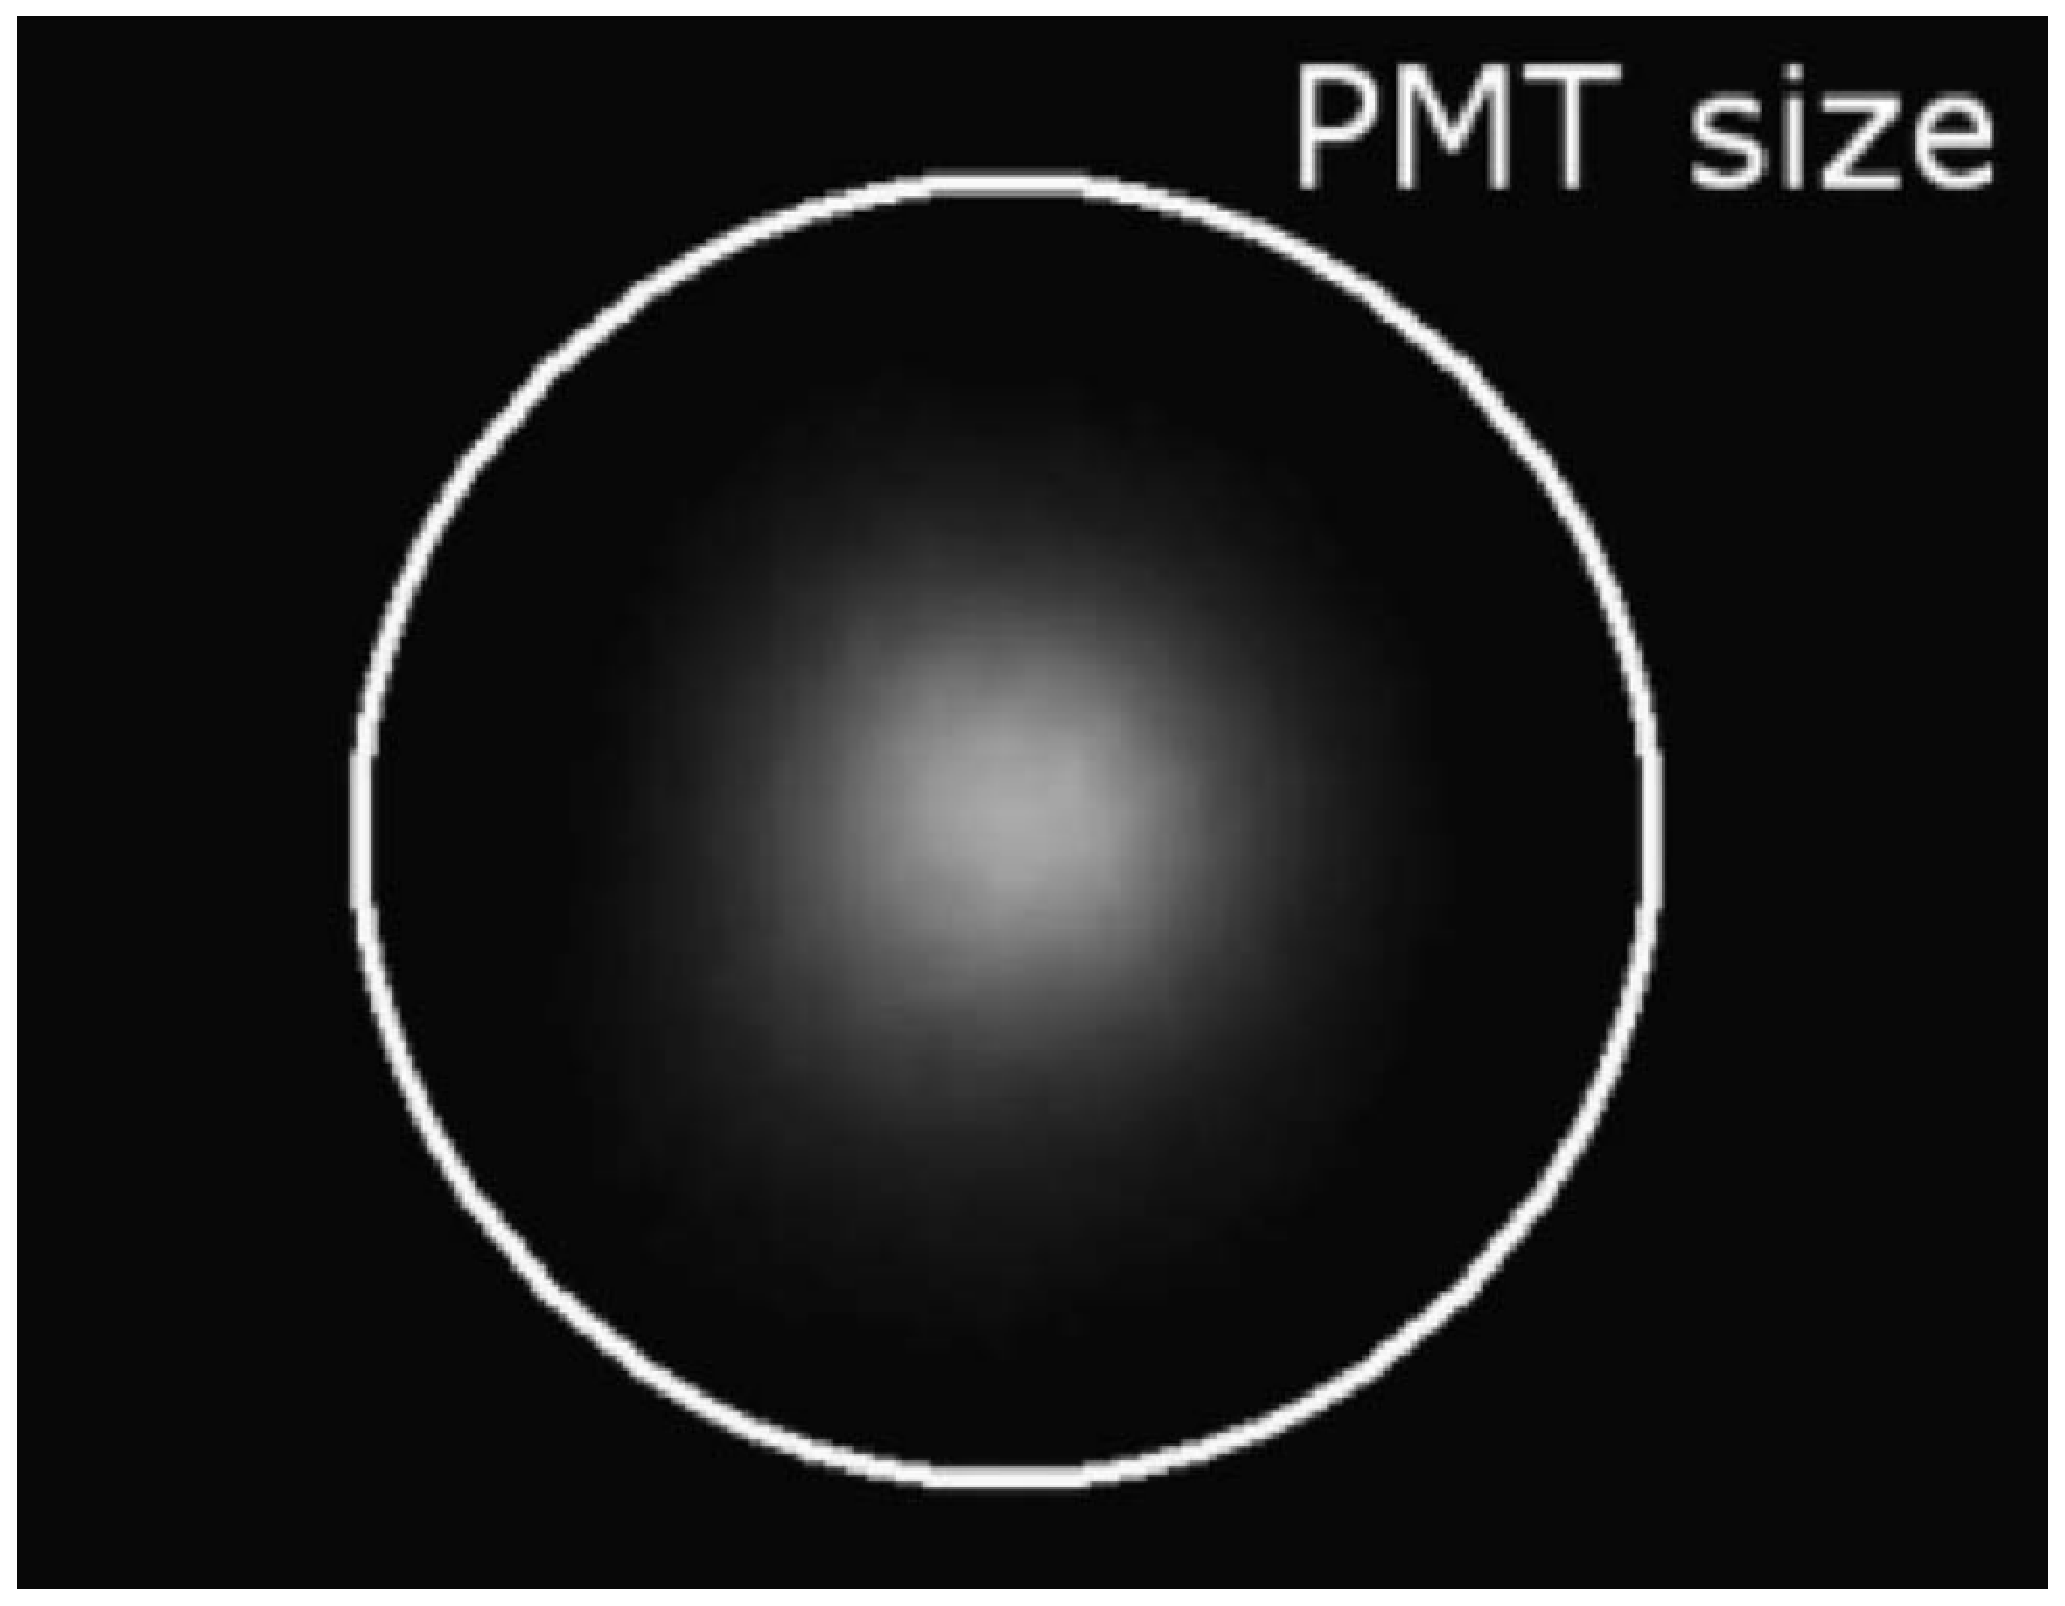
\includegraphics[width=0.75\textwidth]{images/mirror_polaris.eps}
  \caption[Polaris PSF]{
    Image of Polaris after reflecting off the mirrors, demonstrating the shape of the OPSF, from~\cite{Veritas_Detector}.
    The circle indicates the radius of a PMT.}
  \label{fig:mirrorpolaris}
\end{figure}

This point spread function is important, because it determines how accurately cherenkov showers are imaged.
A larger star point spread function means cherenkov images are blurred out, which adds to the gamma-ray point spread function, discussed in Chapter~\ref{ch:grrecon}.
A larger gamma-ray point spread function then blurs out each gamma-ray emitter, making them harder to distinguish from one another.


\subsection{Mirror Alignment}
% https://veritas.sao.arizona.edu/wiki/index.php/Mirror_Alignment
The mirror alignment procedure is performed by placing a CCD camera at the focal plane, facing towards the mirrors.
The telescope is then pointed towards a magnitude 2 star at \nicetilde{}\ang{70} elevation.
The pointing is known as a `raster' scan of the star, where each mirror's field of view is in turn centered on the star.
By using the CCD to examine the position of the star in each mirror, the mirror's alignment can be calculated and corrected.



\section{PMTs}\label{sec:pmts}

Each telescope has a PMT Camera on the end of four supporting arms, inside a protective housing.
This camera consists of 499 Photo Multiplier Tubes (PMTs), each with a Winston cone to increase the light collection area for each PMT~\cite{Winston1970}.
% Winston 1970, Hildebrand and Winston 1982, Hildebrand 1985, Welford and Winston 1989
The PMTs are Hamamatsu's model R10560-100-20 MOD~\cite{pmtmodels}.
These Winston cones can be seen attached to the PMTs in Figure~\ref{fig:winstcones}.

\begin{figure}[ht]
  \centering
  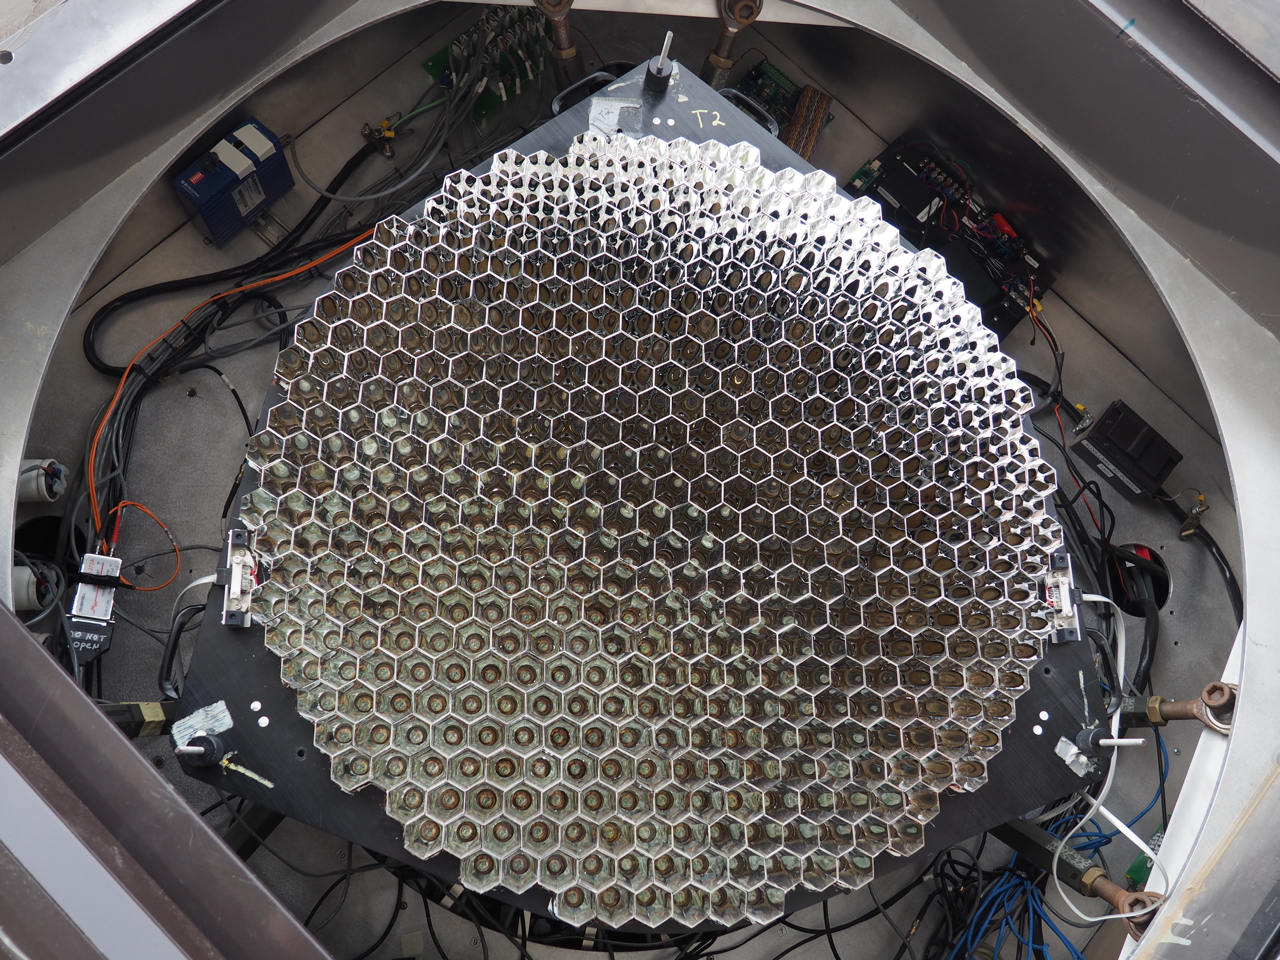
\includegraphics[width=0.75\textwidth]{images/winston_cones_t2}
  \caption[Winston Cones]{
    Hexagonal Winston cones over the circular PMTs, inside the camera housing.}
  \label{fig:winstcones}
\end{figure}


\begin{figure}[ht]
  \centering
  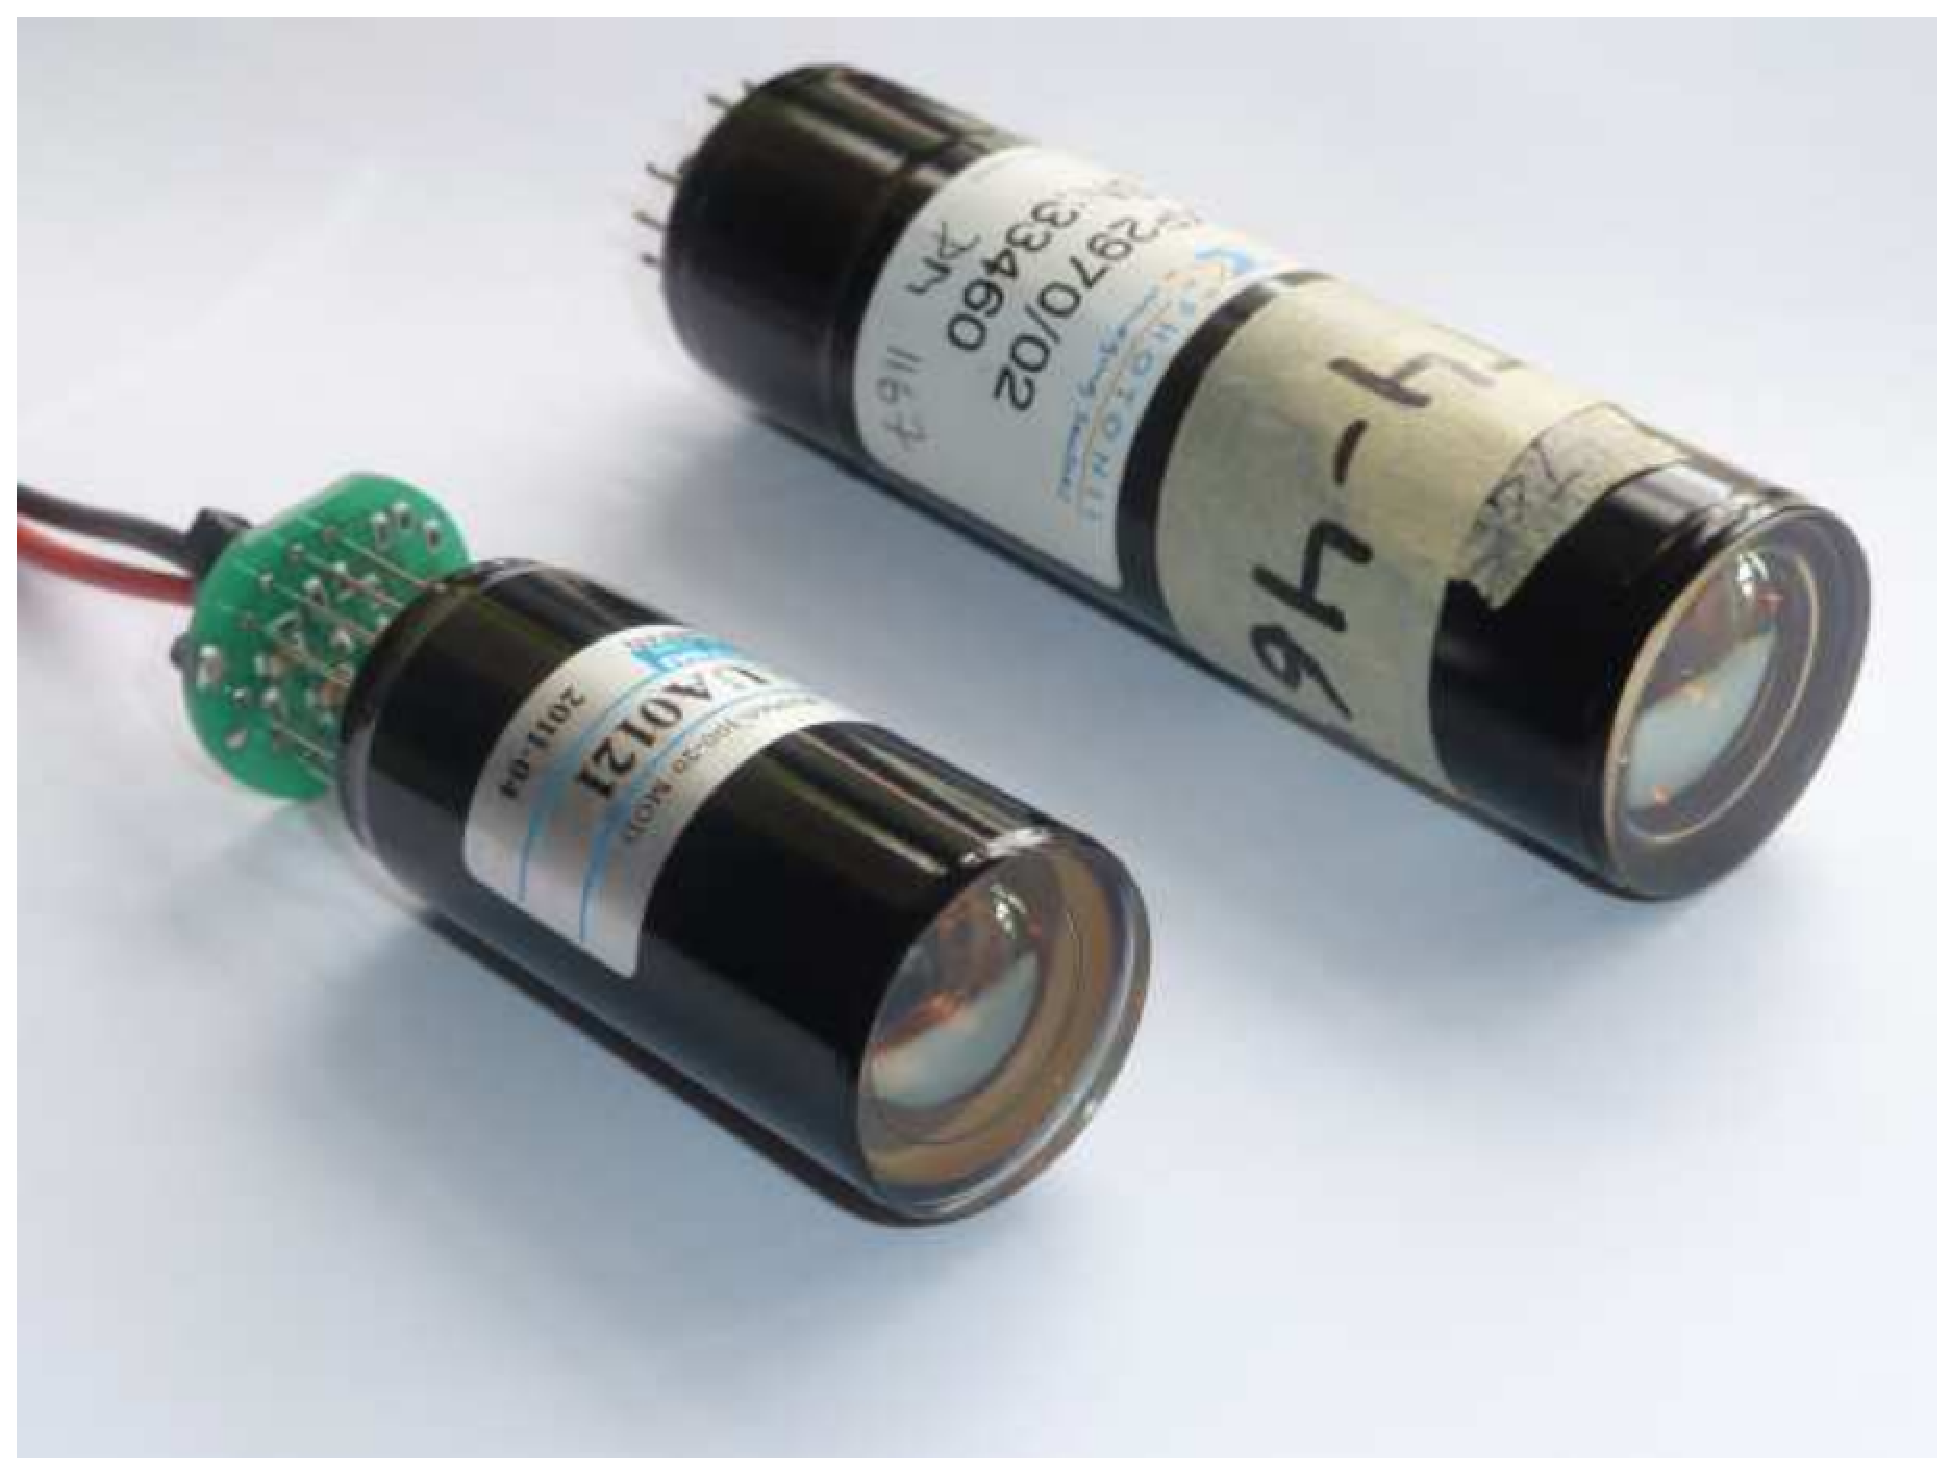
\includegraphics[width=0.75\textwidth]{images/pmt_models/pmt_models}
  \caption[PMT Models]{
    The two PMT models used in the VERITAS cameras~\cite{pmtmodels}.}
  \label{fig:pmtmodels}
\end{figure}

To operate, the PMTs are connected to high voltage, typically \SIrange{900}{1200}{V}.
% mysql -u <username> -h <veritas database> -e "select * from VERITAS.tblHV_Telescope0_Voltages where db_start_time >= '2016-12-01 00:00:00' and db_start_time < '2017-01-30 00:00:00' " >| tmp.txt
% cat tmp.txt | awk '$6>0 {print $6}' | $VERIPY/scripts/hist.py
%
%min      :  275.0
%max      :  1593.0
%mean     :  1054.22
%standev  :  162.73
%elements :  93609
%total    :  98684135.0
%bin width:  131.80
%
%1527 XXX                   6069
%1395 X                      575
%1263 X                     3122
%1131 XXXXXXXXXXXXX        27378
% 999 XXXXXXXXXXXXXXXXXXXX 40171
% 868 XXXXXX               13694
% 736 X                     2437
% 604 X                       14
% 472                      
% 340 X                      149
% mean voltage = 1054, standev = 162, approximate as 1050+-150 = rane of 900-1200
The PMTs' output signals are first sent through an amplifier, before travelling down a \nicetilde{}\SI{45}{m} cable to trigger and digitization electronics stationed near the telescope.

The first circuit that the signal passes through is a Constant Fraction Discriminator (CFD) circuit~\cite{cfd_behavior}.
This circuit's behavior, shown in Figure~\ref{fig:cfd_operation}, duplicates the signal voltage pulse from the PMTs, inverts and delays the duplicate pulse, and adds it back to the original pulse.
This combined pulse then sent to a Zero Crossing Discriminator (ZCD), which emits a \SI{10}{ns} trigger pulse when it crosses the zero-volts threshold.
% theres also CFD Design Review Jun 2001: http://www.if.pw.edu.pl/~alice/CFD7.pdf , slide 12

\begin{figure}[ht]
  \centering
  \includegraphics[width=0.95\textwidth]{images/cfd_operation/cfd_operation.pdf}
  \caption[CFD Operation]{
    CFD signal processing, from Ref.~\cite{cfd_operation}.
    An input signal on the left is manipulated to allow for constant fraction discrimination.
  }
  \label{fig:cfd_operation}
\end{figure}

The use of this circuit has two main benefits.
The first is that the CFD circuit will trigger at the same position within the pulse, regardless of the pulse's size.
If a simple voltage-threshold trigger is instead used, the time of the trigger will be earlier for faster-rising large pulses, and later for slower-rising small pulses.
The CFD's zero threshold trigger is invoked when the signal voltage pulse is reaches a predetermined fraction of its maximum value.
For VERITAS, this fraction threshold is set at 75\% of its maximum value.
% griffin 2016 thesis, page 47, figure 3.17 caption
The second benefit is that when the CFD circuit detects a voltage pulse larger than a given maximum threshold, it can emit an extra logic trigger, called a low-gain trigger.
This extra low-gain trigger is then used by the Flash Analog-to-Digital Circuit (FADC) to switch between high-gain and low-gain mode when digitizing voltage pulses.

Stars and other sources of background light emit background visible photons (Night Sky Background or NSB photons) that can falsely trigger the CFD circuit, contaminating any Cherenkov signals.
In order to reduce this contamination, the CFD circuit is set to ignore any pulses smaller than 50mV.
This threshold is adjusted during observations to account for varying rates of NSB photons.

After the CFD emits a trigger pulse, the signal voltage pulse is passed to the FADC circuit for digization.
This FADC circuit then, for each 2-nanosecond time bin, measures how large the voltage pulse is with a series of 255 voltage thresholds.
% see Bird 2015 thesis, page 52, top line
% time bin = 2ns, stored in an 8-bit int, so 256 possible values, or 255 values + a 0 value
The highest threshold that is crossed in a single time bin then determines the digital voltage value that is saved to the FADC buffer for that time bin.

{\color{red}(?? Please read the T1 paper again, the following paragraph is not entirely correct -Gernot)}
If the low-gain trigger pulse was also recieved by the FADC, then the signal voltage pulse is de-amplified {\color{red}(means attenuated, or reverse the effect of the previous amplification??)} before being digitized, since the CFD low-gain threshold is set lower than the FADC maximum digitizable voltage.
If this low-gain triggering did not take place, then the FADC would become saturated.
Once the voltage pulse is digitized, it is saved to a rolling buffer {\color{red}(how long is the buffer??)} in the FADC, waiting for higher level triggers, signaling the FADC to readout its buffers into a datafile.

\subsection{PMT Upgrade}
In summer of 2012, all PMTs in the telescopes were replaced with improved PMTs.
Specifically, the original Photonis XP2970 models were replaced with the Hamamatsu R10560-100-20 MOD.
This was done because that R10560 has a considerably higher collection rate of Chernekov photons (35\%), compared to the XP2970 (23\%).
This higher collection rate means more photons from a shower are detected by the PMT, which makes VERITAS more sensitive to lower energy gamma rays.
In addition, single-photoelectron studies indicate the R10560's voltage pulse FWHM is \nicetilde{}40\% shorter than the XP2970, as shown in Figure~\ref{fig:pmt_pulse_widths}.
These thinner voltage pulses allow for easier discrimination between NSB fluctuations and Cherenkov signals~\cite{pmtmodels}.

\begin{figure}[ht]
  \centering
  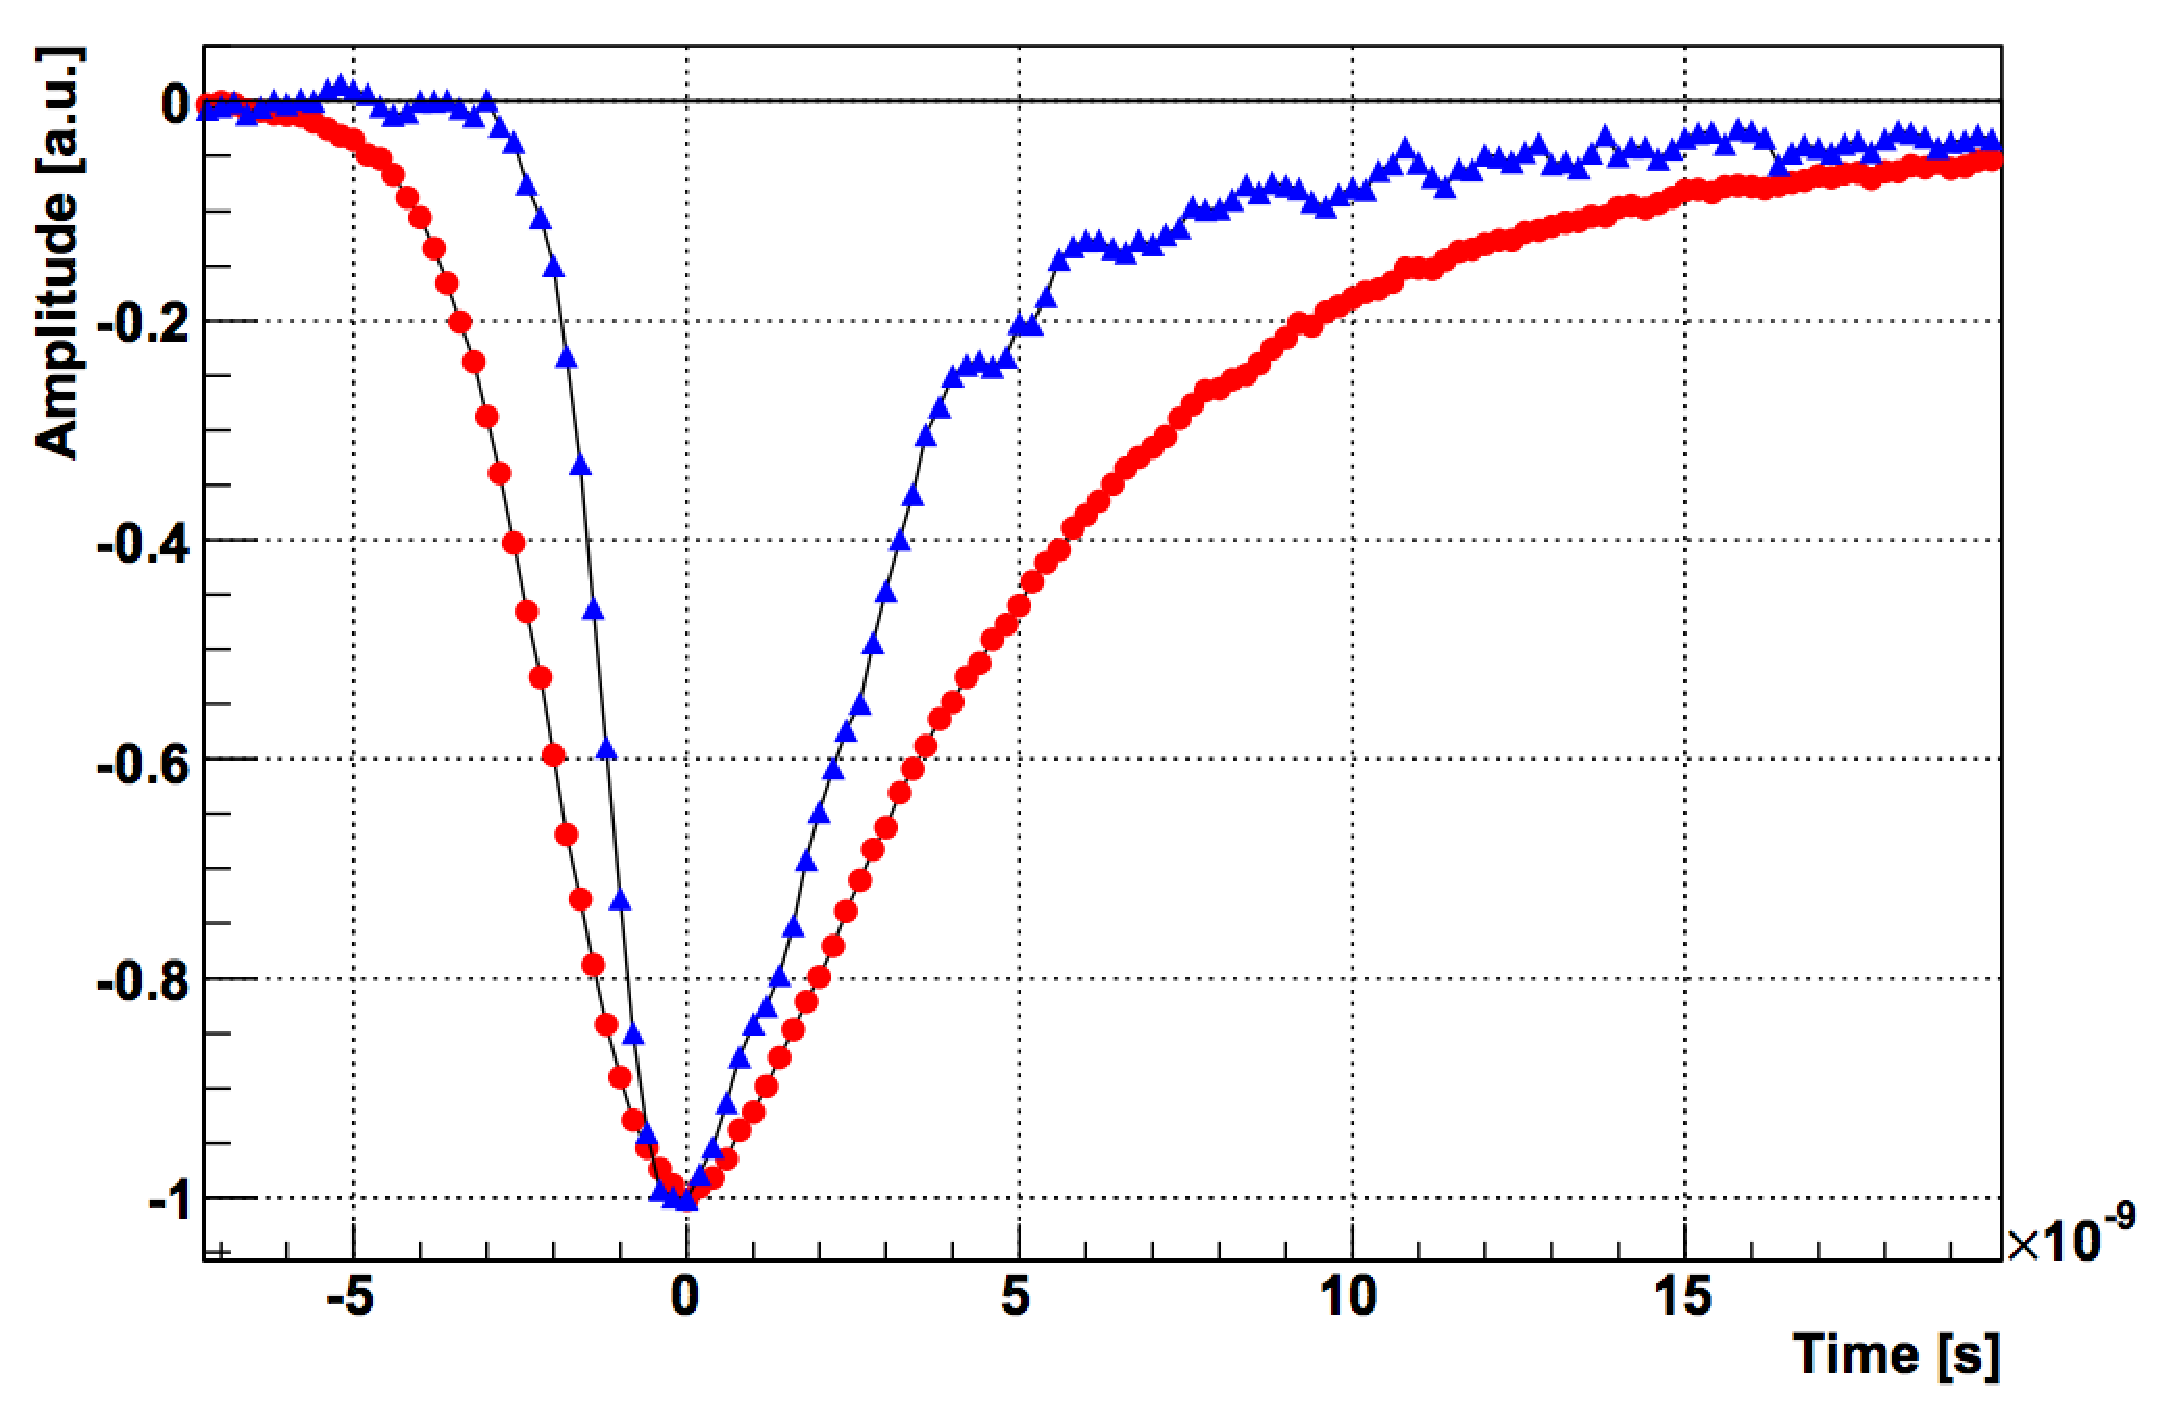
\includegraphics[width=0.75\textwidth]{images/pmt_models/pmt_models_pulsewidths.eps}
  \caption[Pulse Shapes]{
    Pulse shapes of the old XP2970 PMTs (red circles) and the new R10560 PMTs (blue triangles)~\cite{pmtmodels}.
    Plots are the average of many afterpulses, normalized to the maximum amplitude.
    Pulses shown include dispersion due to a \nicetilde{}\SI{55}{m} coaxial cable between the PMTs and the digitizer boards.}
  \label{fig:pmt_pulse_widths}
\end{figure}

The data used in this thesis was taken both before and after this upgrade, which means the telescope performance is different for these two time periods.
This is accounted for by separate simulations for each PMT model, mostly resulting in different effective areas at the lower energies.
These epochs are discussed further in Section~\ref{sec:epochs}.


\subsection{PMT Calibration}

While the VERITAS PMTs are all the same model, there are still differences from PMT to PMT that can impact any data taken.
Primarily, these differences can cause the same number of incident photons to create differently-shaped output voltage pulses in each PMT.
To account for these differences, there a calibration procedure that is applied nightly or semi-nightly.
These are performed with a set of flashing LEDs, placed next to the mirrors such that they illuminate the PMTs.

Once every few nights the single-photoelectron curves for each PMT are measured.
This is done by placing an opaque (several-mm-thick metal) plate over the PMTs, with a mm-diameter hole drilled over the location of each PMT.
The LEDs are then flashed repeatedly.
As the opaque plate has holes for each PMT, each PMT gets on average \SIrange{0}{5} photons per flash.
Large numbers of flashes can then be used to gather information on each PMTs' distribution of pulse widths.
By examining a histogram of the pulses' integrated charges, one can see poisson-statistics peaks that are formed for the 1, 2, 3, and further integer numbers of photons.
These peaks can then be used to translate the digital counts from the PMTs into their originating photoelectrons.
These calibration techniques are further detailed in Ref.~\cite{calib_techniques}.


\section{Trigger System}\label{sec:trig}

The operation of VERITAS requires digitizing voltage pulses with voltage samples roughly once per nanosecond, per photomultiplier tube.
This means that, with 255{\color{red}(??)} voltage levels, 1 second of raw voltage data would require 2 Terabytes of harddrive space.
Since this is unfeasable with today's computing systems, only subsets of the raw pixel voltages are saved when certain trigger conditions are met.
To complicate matters, photons from atmospheric muons and the night sky background can also cause voltage pulses similar to a gamma ray shower's cherenkov photons.
Thus, VERITAS has a system of triggers that reduces the amount of raw data that is saved, while also partially filtering out non-gamma-ray events.

The L1 is the first and lowest level trigger.
An L1 trigger (sometimes called a pixel trigger) is emitted when a PMT's CFD circuit detects a signal voltage above a given threshold, typically in the 10s of mV.
This threshold voltage is varied throughout data taking by a rate-feedback system, which adjusts the trigger threshold according to the night sky background level.

{\color{red}((??) Again, this paragraph is far too detailed and not relevant -Gernot)}
{\color{red}((??) this paragraph does not connect to the ones above and below -Parents)}
The L2 (image) trigger is emitted by the FPGA when a group of L1 triggers meet certain requirements.
These requirements include that multiple L1 triggers must fall within a certain time window, and that multiple L1 triggers form one of several predefined shapes, or templates.
The coincident time window varies. {\color{red}(elaborate??)}
There are several patterns. {\color{red}(elaborate??)}
The pattern requirements help reduce the number of triggers from non-gamma-ray sources.
Night sky background photons are only able to trigger individual pixels, and muons tend to create ring-shaped images.
Once one of these patterns occurs within a time window, the FPGA emits an L2 trigger, which is sent to the L3 (array) trigger system.

{\color{red}(check for any 'a \nicetilde`, there should be no article!??)}
The L3 (array) trigger system is a computer which looks for coincident L2 triggers that fall within \nicetilde\SI{50}{ns} time window.
This window is varied for each telescope based on the azimuth and elevation of the pointing, as these can introduce delays between images of up to hundreds of nanoseconds.
During a typical observation period, the L3 trigger rate is around \SIrange{200}{300}{Hz}.

Once an L3 trigger is invoked, a signal is sent to all telescopes that directs the digitized voltages for all pixels in the cameras to be read out from their buffers, and saved to memory.
These pixel voltages are then processed by the analysis software to reconstruct the gamma-ray events.



\subsection{Deadtime}
When the L3 trigger is invoked and the buffers are being read out, the FADCs are unable to store new PMT voltages in the buffers.
Being unable to store new PMT voltages effectively reduces the amount of time spent observing gamma rays.
This lost time is usually referred to as deadtime.
As the deadtime is a fixed time loss per event, the percent of time lost due to event readout rises with the a higher frequency of readouts.
This means that at an L3 trigger rate of \nicetilde{}\SI{300}{Hz}, approximately \nicetilde{}12\% of the time is lost due to buffer readouts.
Since the L3 rate varies over the course of a single 30 minute run, this means that the deadtime also varies, and is accounted for in Chapter~\ref{chapter:analysis}.

\subsection{Time Zero Calibration}
As all PMTs and signal cables are not identical, there are differences in how long a voltage pulse takes to travel.
More specifically, the time between a) when the photon strikes the PMT's photocathode and b) when the voltage pulse sets off its L1 trigger, can vary from pixel to pixel.
This is usually measured by looking at the average arrival time of many events over all camera pixels.
By looking at the average arrival time, pixels that are consistantly early or late can be accounted for, which improves image identification.

\section{Epochs}\label{sec:epochs}
Since it was completed in 2007, VERITAS has evolved over several years as collaboration members have upgraded it to improve its performance.
However, these major differences need to be taken into account in the analysis chain.
To organize these differences, in the data they are referred to as epochs 1, 2, 3, 4, 5, and 6 (usually denoted as V1, V2, V3, V4, V5, and V6).
The four telescopes were built within a coordinate system where the origin is at 31.675N, 110.962W, the x axis points East, and the y axis points North.

As the first three telescopes were constructed and brought online, data taken after each is considered part of the first, second, and third epochs.
Telescope 1 was placed at (-37.6, -23.7), telescope 2 at (44.1, -47.7), and telescope 3 at (29.4, 60.1).
In 2007, the fourth telescope was constructed at (-35.9, 11.3), and data taken between this point in time and the next major upgrade is considered the fourth epoch (V4).

In September 2009, telescope 1 was moved to a new position (135.4, -8.61), after it was demonstrated with simulations that it would grant a \nicetilde{}30\% improvement in sensitivity~\cite{veritas_t1_move}.
Data taken after this relocation is referred to as the fifth epoch (V5).

In August 2012, the PMTs in all cameras were replaced with improved PMTs that had a higher quantum efficiency, improving the telescopes ability to resolve images~\cite{pmtmodels}.
Data taken after this upgrade is considered part of the sixth epoch (V6).

As these different epochs have different telescope configurations, the instrument response functions are different, meaning each epoch behaves in a quantifiably distinct manner.
For the Dark Matter analysis described in this thesis, only data from the fifth and sixth epochs are used, detailed further in Table \ref{tab:observation_times}.


